\chapter[Sweeper]{Sweeper: ejecución de flujos de trabajo en cómputo en la nube}
\label{chap:sweeper}

En este capítulo se describen los detalles del funcionamiento de Sweeper \cite{dominofire2015sweeper}, el sistema de administración de flujos de trabajo orientado a cómputo en la nube. Utilizando este paquete, se pueden ejecutar tareas expresadas como comando de una terminal Linux, con dependencias de orden entre ellas entre recursos en la nube. Sweeper está desarrollado en el lenguaje de programación Python \cite{python3}.

Para ejecutar flujos de trabajo con Sweeper, se especifican las tareas del flujo de trabajo y sus dependencias. Sweeper lee este archivo de descripción y enseguida estima los tiempos de ejecución de las tareas y elige la mejor asignación de máquinas virtuales y tareas del flujo de trabajo que optimicen los criterios dados.

Para crear un flujo de trabajo, se crea un archivo que cumpla con el formato YAML



\section{Arquitectura}

En figura \ref{fig:sweeper-arch} se muestra la arquitectura de Sweeper, en donde se pueden notar cuatro grandes componentes: la ejecucíón del flujo de trabajo, el planificador, el perfilador de las tareas y el perfilador de los recursos. Sweeper utiliza las interfaces de programación de aplicaciones de cada proveedor de servicios de cómputo en la nube para reservar, ejecutar y administrar los recursos utilizados en la nube de cada proveedor. Actualmente, Sweeper puede trabajar con los servicios de cómputo en la nube de Microsoft Azure \cite{microsoft2015azure}. En las siguientes subsecciones, describiremos a detalle cada uno de los componentes de Sweeper.

\begin{figure}
\begin{center}
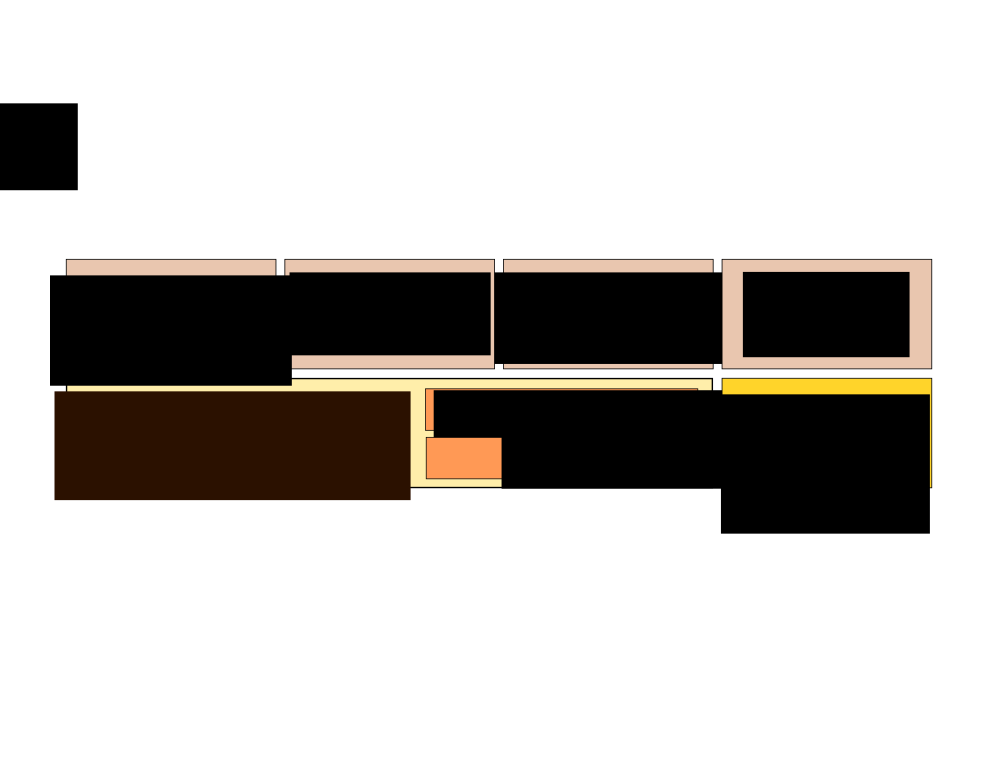
\includegraphics[width=0.8\textwidth]{imagenes/sweeper-architecture.pdf}
\end{center}
\caption{Arquitectura de Sweeper}
\label{fig:sweeper-arch}
\end{figure}


\subsection{Ejecución de flujos de trabajo}

Este componente se encarga de ejecutar el flujo de trabajo en los recursos en la nube de acuerdo a la planificación generada por el componente de planificación. Por el momento, este componente implementa un sistema de colas concurrente en las que las tareas son insertadas y despachadas de acuerdo al tiempo de ejecución estimado.



\subsection{Planifcador}

El planificador busca la asignación de recursos que optimice la calidad en el servicio en la ejecución del flujo de trabajo, interpretado como restricciones de presupuesto o restricciones de fechas límite. 



\subsection{Perfilador de tareas}



\subsection{Perfilador de recursos}
